% Created 2019-01-15 Tue 14:31
\documentclass[11pt]{article}
\usepackage[utf8]{inputenc}
\usepackage[T1]{fontenc}
\usepackage{fixltx2e}
\usepackage{graphicx}
\usepackage{longtable}
\usepackage{float}
\usepackage{wrapfig}
\usepackage{rotating}
\usepackage[normalem]{ulem}
\usepackage{amsmath}
\usepackage{textcomp}
\usepackage{marvosym}
\usepackage{wasysym}
\usepackage{amssymb}
\usepackage{hyperref}
\tolerance=1000
\usepackage{minted}
\usepackage{amsthm}
\usepackage[margin=1.0in]{geometry}
\setlength{\parindent}{0pt}
\setlength{\parskip}{\baselineskip}
\author{Thomas Alford}
\date{\today}
\title{Ph21 Problem Set 1}
\hypersetup{
  pdfkeywords={},
  pdfsubject={},
  pdfcreator={Emacs 25.2.1 (Org mode 8.2.10)}}
\begin{document}

\maketitle

\section*{Introduction}
\label{sec-1}

Here we are looking at data from the Catalina Real-Time Transient
Survey. Earlier in the set, the website
\url{http://nesssi.cacr.caltech.edu/cgi-bin/getcssconedbid_release2.cgi} was searched
manually for the Her X-1 binary system. This is the plot the website generated
in terms of intensity over time:

[[\includegraphics[width=.9\linewidth]{/Users/tommyalford/Desktop/Ph21Set1HerX1.png}]]


We will now attempt to recreate this plot by accessing the website data using
python. We will parse the data first using string methods and next using
astopy.io.votable.

\section*{Imports}
\label{sec-2}
\begin{minted}[frame=lines,fontsize=\scriptsize]{python}
import numpy as np
import matplotlib.pyplot as plt
import seaborn as sns
import urllib.request
from astropy.io.votable import parse
sns.set(font_scale=1.5)
\end{minted}

\section*{Reading in the Data}
\label{sec-3}
These value querys were found by inspecting the source code of website,
checking the values of 'name =' fields:

\begin{minted}[frame=lines,fontsize=\scriptsize]{python}
url = 'http://nesssi.cacr.caltech.edu/cgi-bin/getcssconedbid_release2.cgi'
values = {"Name": "Her X-1", "SHORT": "short", "DB": "photcat", "OUT": "web",
          "Rad": .1}
data = urllib.parse.urlencode(values)
data = data.encode('ascii') # data should be bytes
with urllib.request.urlopen(url, data) as response:
   html = response.read()
\end{minted}


Now we need to decode this to convert it back to a string:
\begin{minted}[frame=lines,fontsize=\scriptsize]{python}
data_str = html.decode('ascii')
\end{minted}

\section*{Parsing the Output Using String Methods}
\label{sec-4}

Here we find that the real table begins somewhere in the middle of the file,
after a </tr><tr><td> tag combination. We'll truncate this and see what we get:

\begin{minted}[frame=lines,fontsize=\scriptsize]{python}
ind_str = '</tr><tr><td>'
trunced_data = data_str[data_str.index(ind_str):]
\end{minted}


\begin{minted}[frame=lines,fontsize=\scriptsize]{python}
print(trunced_data[:1000])
\end{minted}

\begin{verbatim}
</tr><tr><td>1135075<td> 253.01875<td> 35.27778<td> 1<td> 2.8<td> 251.246<td> 254.795<td> 33.8423<td> 36.7</tr>
</table><br><p><table bgcolor="#c0c0c0" border><tr><Caption>Master Objs in Region</Caption></tr><tr><th>OBJ ID<th>Mag<th>RA<th>Dec<th>Offset (")</tr><tr><td>1135075045477<td>13.355<td>254.45751<td>35.342352<td>   0.19</tr>
</table><br><p>
<table border=1 width=500 bgcolor="#c0c0c0"><tr><Caption>Photometry of Objs:</Caption></tr><tr><th>OBJ ID<th>Mag<th>Magerr<th>RA<th>Dec<th>MJD</tr><tr><td>1135075045477<td>13.34<td>0.05<td>254.4576<td>35.3424<td>53557.32593</tr>
<tr><td>1135075045477<td>13.34<td>0.05<td>254.4575<td>35.3423<td>53557.33004</tr>
<tr><td>1135075045477<td>13.34<td>0.05<td>254.4575<td>35.3424<td>53557.33418</tr>
<tr><td>1135075045477<td>13.32<td>0.05<td>254.4576<td>35.3424<td>53557.33834</tr>
<tr><td>1135075045477<td>13.51<td>0.05<td>254.4575<td>35.3423<td>53562.24598</tr>
<tr><td>1135075045477<td>13.50<td>0.05<td>254.4575<td>35.3423<td>53562.25304</tr>
<tr><td>11
\end{verbatim}

Here we see about four sections separated by newline characters before getting
to the actual Photometry data table. So we just need to split over the newline
character and then take all the elements beyond:

\begin{minted}[frame=lines,fontsize=\scriptsize]{python}
table_data = trunced_data.split('\n')[4:]
\end{minted}


Let's check out the data now:

\begin{minted}[frame=lines,fontsize=\scriptsize]{python}
table_data[:10]
\end{minted}

\begin{verbatim}
  ['<tr><td>1135075045477<td>13.34<td>0.05<td>254.4575<td>35.3423<td>53557.33004</tr>',
  '<tr><td>1135075045477<td>13.34<td>0.05<td>254.4575<td>35.3424<td>53557.33418</tr>',
  '<tr><td>1135075045477<td>13.32<td>0.05<td>254.4576<td>35.3424<td>53557.33834</tr>',
  '<tr><td>1135075045477<td>13.51<td>0.05<td>254.4575<td>35.3423<td>53562.24598</tr>',
  '<tr><td>1135075045477<td>13.50<td>0.05<td>254.4575<td>35.3423<td>53562.25304</tr>',
  '<tr><td>1135075045477<td>13.50<td>0.05<td>254.4575<td>35.3423<td>53562.26014</tr>',
  '<tr><td>1135075045477<td>13.48<td>0.05<td>254.4575<td>35.3423<td>53562.26718</tr>',
  '<tr><td>1135075045477<td>13.71<td>0.05<td>254.4575<td>35.3423<td>53526.30884</tr>',
  '<tr><td>1135075045477<td>13.69<td>0.05<td>254.4575<td>35.3423<td>53526.31949</tr>',
  '<tr><td>1135075045477<td>13.67<td>0.05<td>254.4575<td>35.3423<td>53526.32984</tr>']
\end{verbatim}

Here we see that we just need to take out the <tr>s and <td>s found in each line:
\begin{minted}[frame=lines,fontsize=\scriptsize]{python}
def parse_line(table_line):
    splitted = table_line.split('<td>')
    # remove first element, which is just <tr>
    tr_rem = splitted[1:]
    # get rid of </tr> from the last element
    tr_rem[-1] = tr_rem[-1].strip('</tr>')
    # make every item a float
    return list(map(float, tr_rem))
\end{minted}


\begin{minted}[frame=lines,fontsize=\scriptsize]{python}
parse_line(table_data[1])
\end{minted}

\begin{verbatim}
[1135075045477.0, 13.34, 0.05, 254.4575, 35.3424, 53557.33418]
\end{verbatim}

Looks like the parser works. Now we can just parse over the whole table. But,
the end of data has some other elements not from the table, so we need to check
and see which lines only contain the table.

\begin{minted}[frame=lines,fontsize=\scriptsize]{python}
table_data[-4:]
\end{minted}

\begin{verbatim}
  ['<tr><td>1135075045477<td>14.45<td>0.05<td>254.4576<td>35.3424<td>56588.10323</tr>',
  '</table><br><p>',
  '<p><br><p></HTML>',
  '']
\end{verbatim}

So, we'll parse over everything but the last 3 lines:

\begin{minted}[frame=lines,fontsize=\scriptsize]{python}
parsed_data = np.array(list(map(parse_line, table_data[:-3])))
\end{minted}


Now, in np-array form, we can just pull out the magnitude, uncertainties, and
times of each line from the headers in the HTML code earlier:

\begin{minted}[frame=lines,fontsize=\scriptsize]{python}
mags = parsed_data[:, 1]
uncerts = parsed_data[:, 2]
MJDs = parsed_data[:, 5]
\end{minted}

\subsection*{Plotting the Parsed Data}
\label{sec-4-1}

Now, we just need to plot this with error bars:

\begin{minted}[frame=lines,fontsize=\scriptsize]{python}
def plot_mag_data(mags, magerrs, MJDs):
    plt.figure(figsize=(12, 5))
    plt.errorbar(MJDs, mags, color='black', yerr=magerrs, fmt='o', markersize=3,
                ecolor='r', capthick=2)
    plt.gca().invert_yaxis()
    plt.xlabel('Date (MJD)')
    plt.ylabel('V mag')

plot_mag_data(mags, uncerts, MJDs)
plt.title('Light Curves Around Her X-1 at r = .1, String-Parsed')
plt.show()
\end{minted}

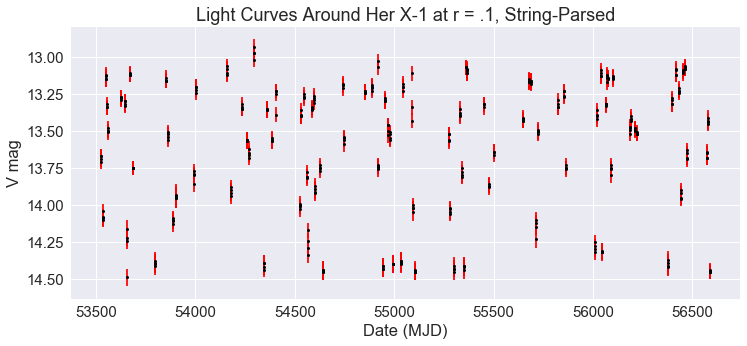
\includegraphics[width=.9\linewidth]{./obipy-resources/17087KNv.png}


\section*{Parsing the data from the XML file in VOTable Format:}
\label{sec-5}

Now we can get the VOtable XML data from online and use the voparser to parser
the data in a much easier fashion:

\begin{minted}[frame=lines,fontsize=\scriptsize]{python}
votable = parse("result_web_fileDR8owK.vot", pedantic=False)
vo_data = votable.get_first_table().to_table()
\end{minted}


\begin{minted}[frame=lines,fontsize=\scriptsize]{python}
vo_data
\end{minted}

\begin{verbatim}
  <Table masked=True length=378>
  MasterID    RAJ2000  DEJ2000  ObsTime [1]  Mag [1]   Magerr [1] Blend [1]
  deg      deg         d
  object     float32  float32    float32    float32    float32     int32
  ------------- --------- -------- ----------- --------- ----------- ---------
  1135075045477 254.45757 35.34235   53557.324 13.338659 0.052161247         0
  1135075045477 254.45753 35.34234    53557.33 13.339489 0.052163184         0
  1135075045477 254.45753 35.34235   53557.336 13.342177 0.052178945         0
  1135075045477 254.45757 35.34235    53557.34 13.324588  0.05213488         0
  1135075045477 254.45750 35.34233   53562.246 13.510649 0.052456874         0
  1135075045477 254.45750 35.34233   53562.254  13.49694 0.052435752         0
  1135075045477 254.45750 35.34231    53562.26 13.500379 0.052439135         0
  1135075045477 254.45750 35.34234   53562.266 13.475543 0.052392595         0
  1135075045477 254.45750 35.34233    53526.31  13.70976 0.052931767         0
  ...       ...      ...         ...       ...         ...       ...
  1135075045477 254.45757 35.34233   56574.137 13.675402  0.05290823         0
  1135075045477 254.45757 35.34234    56574.14 13.675675 0.052921385         0
  1135075045477 254.45753 35.34234   56580.086 13.435135 0.052297443         0
  1135075045477 254.45757 35.34232    56580.09 13.445594 0.052325822         0
  1135075045477 254.45757 35.34232   56580.098  13.42858 0.052298788         0
  1135075045477 254.45755 35.34232   56580.105 13.405985 0.052251775         0
  1135075045477 254.45757 35.34234   56588.082 14.451928  0.05430378         0
  1135075045477 254.45755 35.34236    56588.09 14.453248   0.0543382         0
  1135075045477 254.45757 35.34235   56588.098 14.436412  0.05427364         0
  1135075045477 254.45757 35.34235     56588.1 14.448011 0.054356683         0
\end{verbatim}

Here we see the relevant fields we need to find:

\begin{minted}[frame=lines,fontsize=\scriptsize]{python}
vo_mags = np.array(vo_data['Mag'])
vo_errs = np.array(vo_data['Magerr'])
vo_MJDs = np.array(vo_data['ObsTime'])
\end{minted}

\subsection*{Plotting the VOTable Data}
\label{sec-5-1}

Now we can plot the data just as before:

\begin{minted}[frame=lines,fontsize=\scriptsize]{python}
plot_mag_data(vo_mags, vo_errs, vo_MJDs)
plt.title('Light Curves Around Her X-1 at r = .1, Vo-Parsed')
plt.show()
\end{minted}

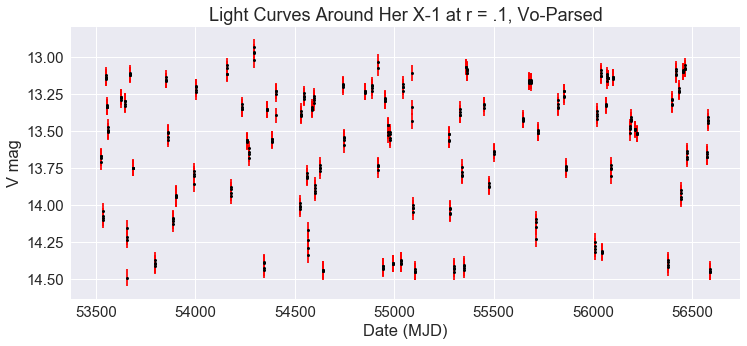
\includegraphics[width=.9\linewidth]{./obipy-resources/17087XX1.png}



Looks like both plots match each other, as well as the plot generated by the website.

\subsection*{Exploring a Period in the Data}
\label{sec-5-2}

Here we'll explore a period of 1.7 MJD in the data by simply modding the date values by 1.7.

\begin{minted}[frame=lines,fontsize=\scriptsize]{python}
plot_mag_data(vo_mags, vo_errs, (vo_MJDs % 1.7))
plt.xlabel('Date mod 1.7 (MJD)')
plt.title('Light Curves Around Her X-1, Exploring a Period of 1.7MJD')
plt.show()
\end{minted}

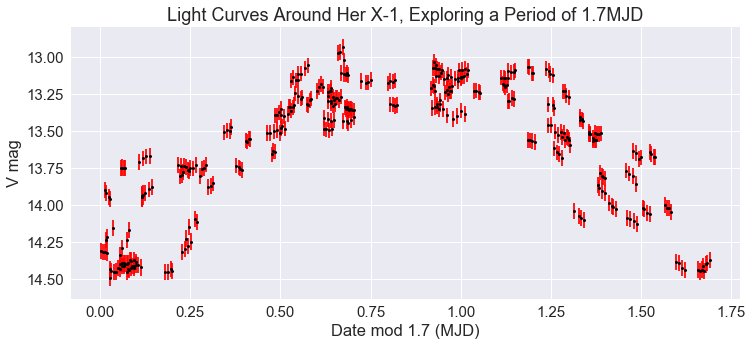
\includegraphics[width=.9\linewidth]{./obipy-resources/17087w_W.png}
% Emacs 25.2.1 (Org mode 8.2.10)
\end{document}
